\documentclass[12pt]{article}
\usepackage{template}
\usepackage{graphicx}
\usepackage{xcolor,listings}
\usepackage{enumerate}
\usepackage{array}

\usepackage{enumitem}
\usepackage{biblatex}
\addbibresource{bib.bib}
\renewcommand{\labelitemi}{$\bullet$}
\renewcommand{\labelitemii}{-}
\author{Fernando López Balcazar}
\begin{document}
\begin{titlepage}
\AddToShipoutPicture*{\BackgroundPic}
\newgeometry{top=1in, bottom=1in, left=1.2in, right=1in}
\begin{spacing}{1.5}
 \begin{figure}[t]
    \centering\includesvg[width=0.3\textwidth]{../Resources/ciencias.svg}
\end{figure}
\begin{center}
	\textsc{\LARGE{Computaci\'on Concurrente\\ }}
	\vspace{15mm}
    \textsc{\LARGE{Equipo Tijeras\\}}
    \vspace{15mm}
	\fontsize{10mm}{7mm}\selectfont
	\textup{Pr\'actica 3 - Spinlocks}\\
	\vspace{20mm}
    \fontsize{8mm}{6mm}\selectfont
    López Balcazar Fernando - 316128182 \\
    Reyes Ramos Luz Mar\'ia - 318211073\\
    S\'anchez Castro Gustavo - 318213888
\end{center}

\vspace{30mm}

\vspace{8mm}
\begin{center}
    \textbf{\large{Fecha de entrega: 5 de octubre de 2023}}
\end{center}
\end{spacing}
\end{titlepage}
\restoregeometry

%%%%%%%%%%%%%%%%%%%%%%%%%%%%%%%%%%
\section{Introducción:}
Zeratun estaba muy contento pues ya pudo recuperar su tanque de gas y sus macetas,
pero se dio cuenta que le roban mucho, por lo que decidio aprender computación
concurrente para que no le pasara de nuevo y asi estar prevenido, ayudemos a zeratun
a aprender computo concurrente y pueda por fin descansar.

\section{Teoría:}
\begin{enumerate}
    \item ¿Para que sirve el método Yield? (yield())\\ \vspace{3mm}

    Sirve para suspender temporalmente la ejecuci\'on de un hilo o proceso. Se suele usar para ceder el control de los procesadores a otros hilos o procesos. Se suele utilizar en situaciones donde se desea evitar que un solo hilo o proceso acapare todos los recursos del sistema.\\ \vspace{3mm}
    
    \item ¿Qué es un atributo átomico? (En la biblioteca atomic de Java)\\ \vspace{3mm}

    Dentro de la biblioteca \textit{atomic} de Java tenemos varias clases como pueden ser \textit{AtomicInteger}, \textit{AtomicLong} y \textit{AtomicBoolean} que nos sirven para crear objetos que nos permitan facilitar la concurrencia e incluso para evitar candados.\\ \vspace{3mm}

    La forma de utilizarlos es creando ejemplares de dichas clases (instancias) las cuales contienen m\'etodos que nos ayudan a evitar el problema de que dos hilos lean una variable y cuando la quieran modificar dicha variable ya haya cambiado, un ejemplo de esto es el ejemplo de que si tenemos un contador entero y hacemos \textit{counter++} si dos hilos tienen acceso a la variable \textit{counter} entonces pueden tener los problemas mencionados anteriormente. Una soluci\'on a esto es en vez de que la variable sea un entero que sea un \textit{AtomicInteger} y en vez de utilizar \textit{counter++} utilizar su m\'etodo \textit{addAndGet(1)} como en el ejemplo \textit{counter.addAndGet(1)}.\\ \vspace{3mm}
    
    \item Ventajas de usar atributos atomicos\\ \vspace{3mm}

    \begin{itemize}
        \item Puedes ahorrarte de utilizar candados.
        \item Evitas resultados inesperados en caso de que no hubieras considerado manejar la concurrencia.
    \end{itemize}
    
    \item Desventajas de usar atributos atómicos\\ \vspace{3mm}

    \begin{itemize}
        \item Estamos trabajando con objetos y no con datos primitivos.
        \item Mayor uso de memoria por lo mismo de que son objetos.
        \item Realizar operaciones m\'as grandes es complicado ya que se necesitan muchos m\'etodos en vez de hacer un simple c\'alculo y reasignarlo.
        \item Se escribe un poco m\'as de c\'odigo.
    \end{itemize}
    
    \item Da 2 ejemplos en donde se puedan aplicar este tipo de atributos.\\ \vspace{3mm}

    En el caso de contadores compartidos por hilos. Tambi\'en podemos utilizarlos para los switch de valores booleanos como el ejemplo de un apagador, podemos cambiar el valor sin preocuparnos de que alguno se anule o incluso que se contrarresten.\\ \vspace{3mm}
    
    \item Algun uso que creas que se da en estructuras de datos concurrentes.\\ \vspace{3mm}

    Para evitar usar variable volátiles y ahorrarnos algunos candados, que aparte de hacer nuestro c\'odigo m\'as sencillo lo hace f\'acil de leer y entender.\\

    
\end{enumerate}
\section{Práctica:}
Para esta parte decidimos usar un graficador y un tabulador que programamos en phyton con lo cual quedaron de la siguiente manera :
 \begin{itemize}

 
     \item Gustavo :
    
     
      \begin{center}
         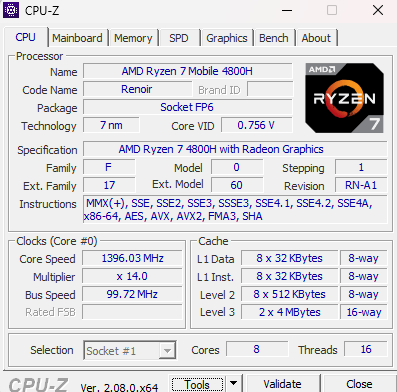
\includegraphics[width=0.6\linewidth]{Practica3//ImaP3/e2.png}
     \end{center}
      \begin{center}
         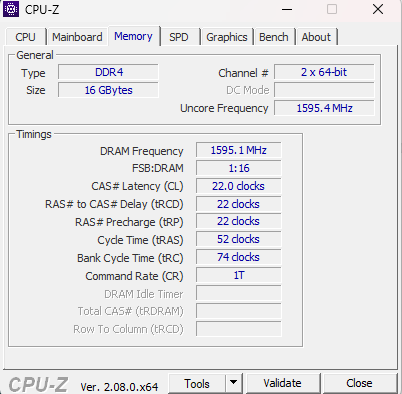
\includegraphics[width=0.6\linewidth]{Practica3//ImaP3/e.png}
     \end{center}
 \begin{center}
         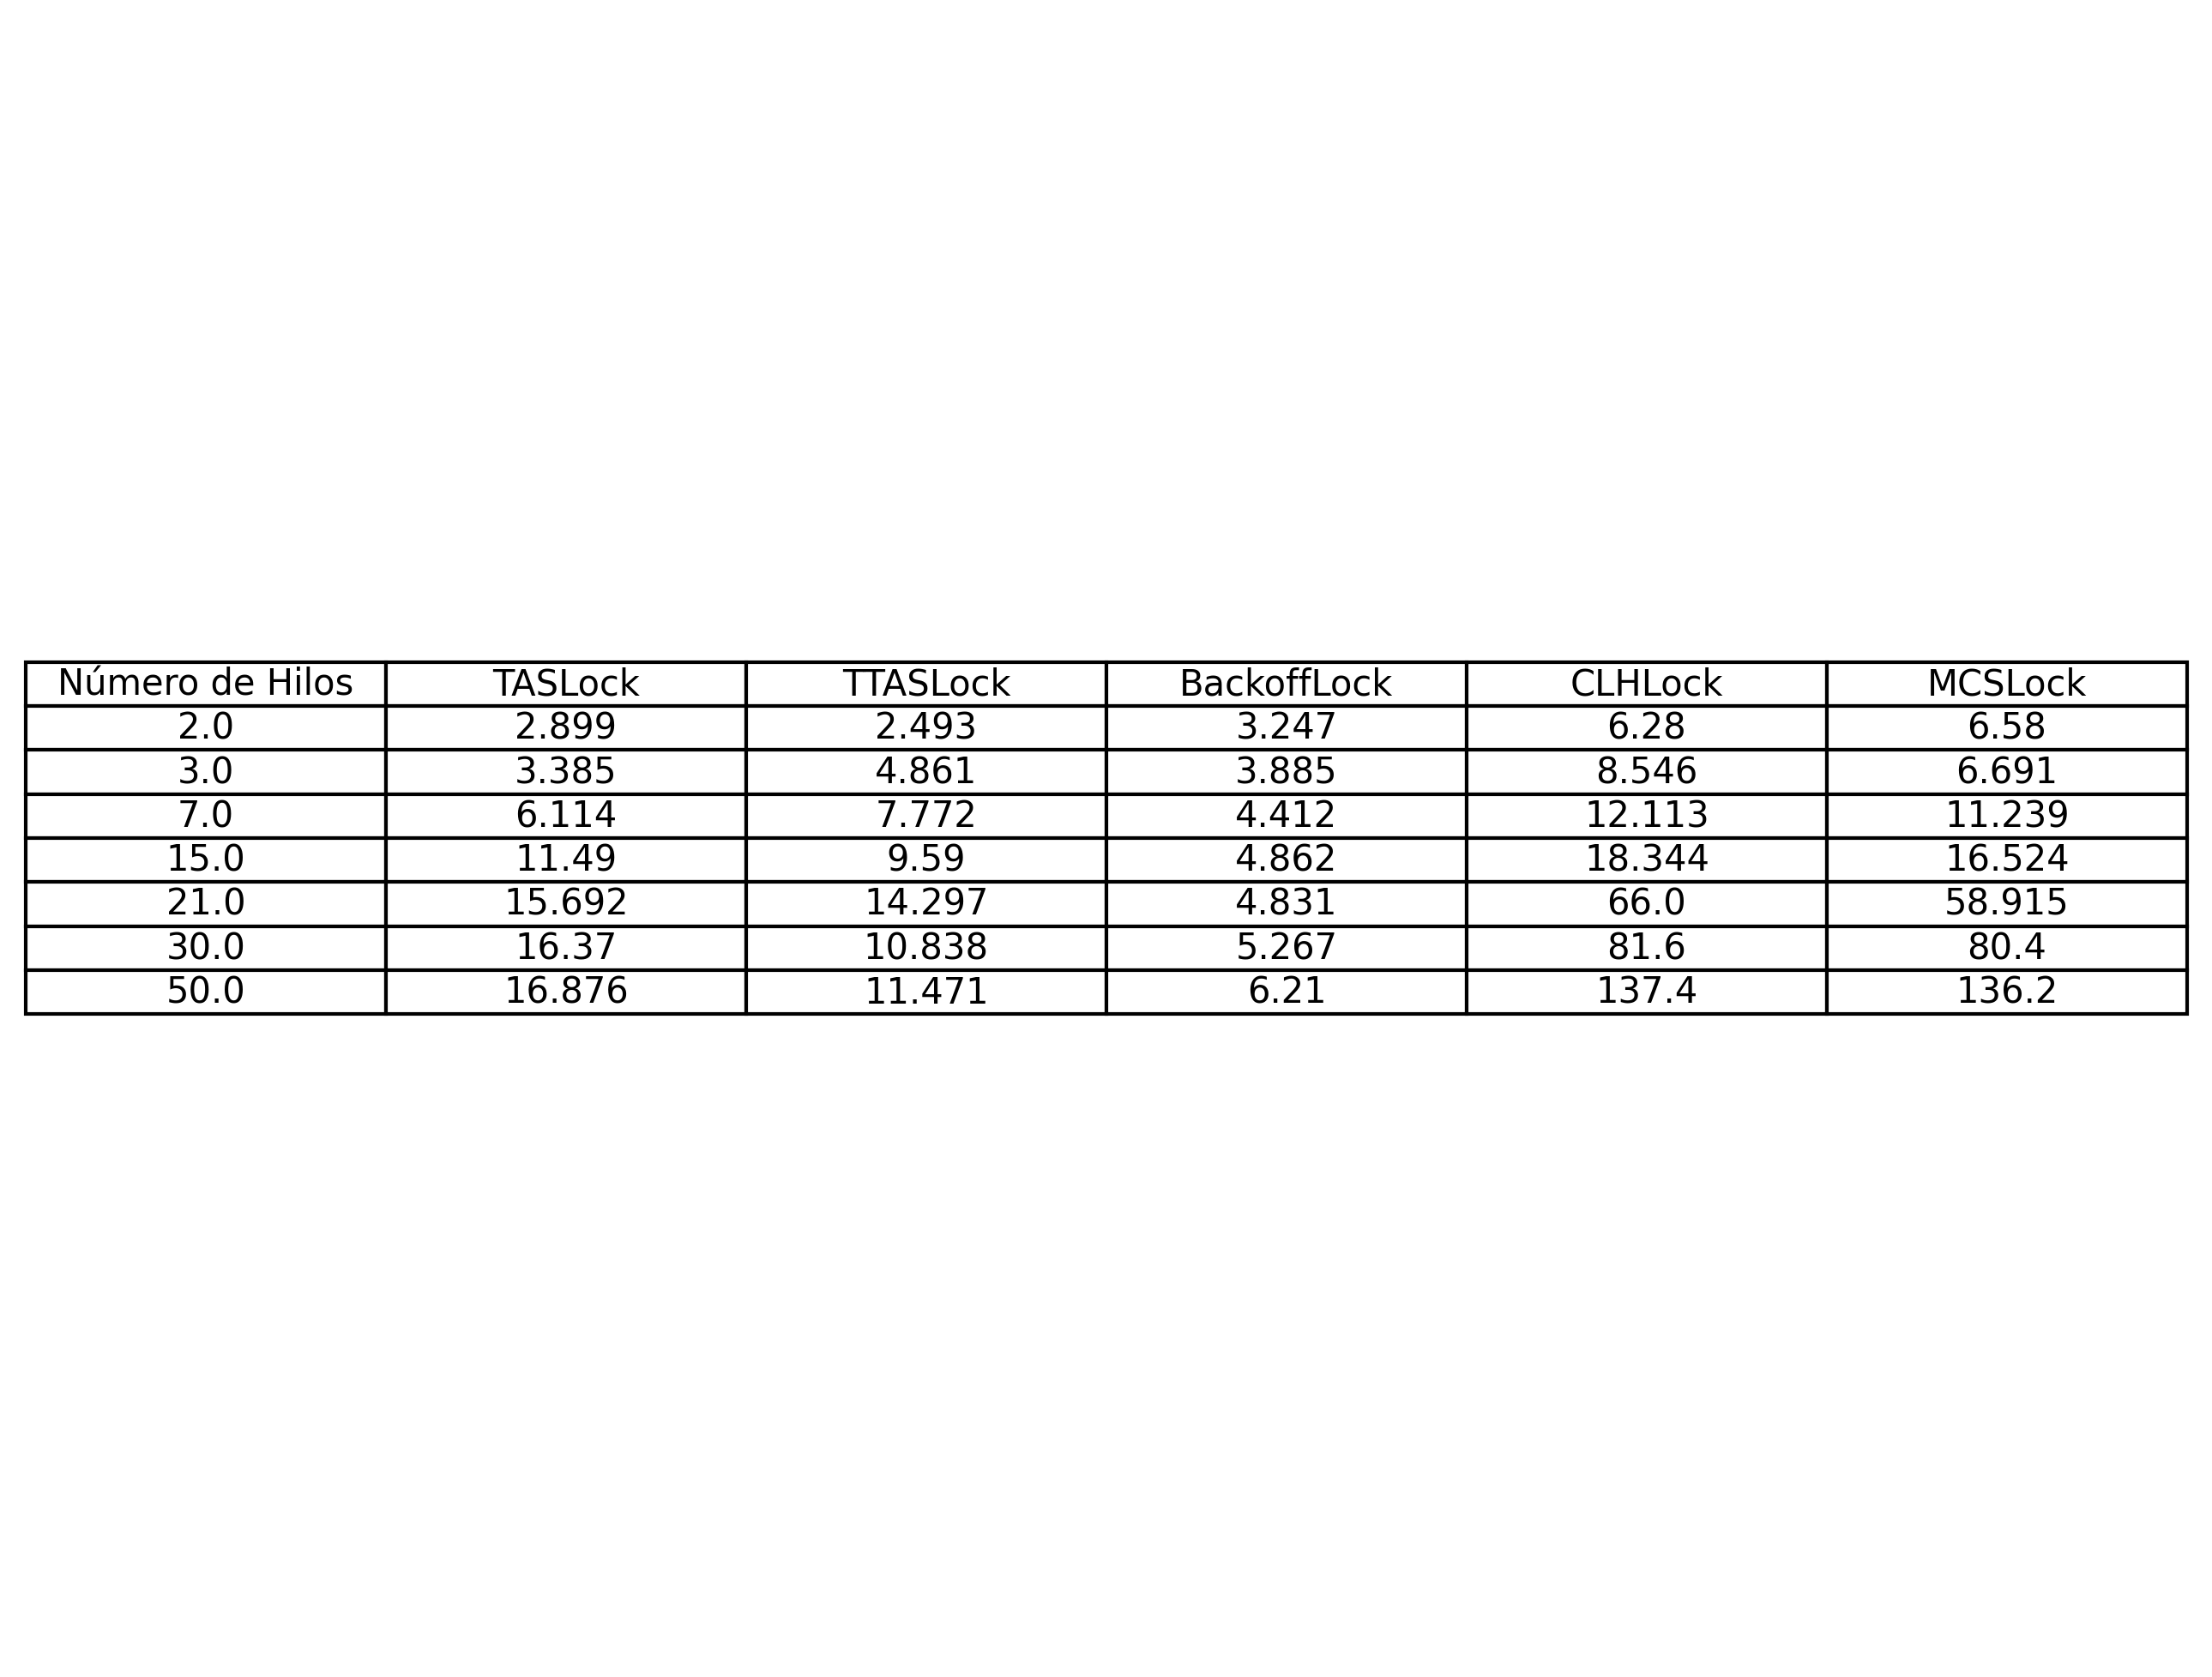
\includegraphics[width=1.0\linewidth]{Practica3/ImaP3/t1.png}
     \end{center}
     \begin{center}
         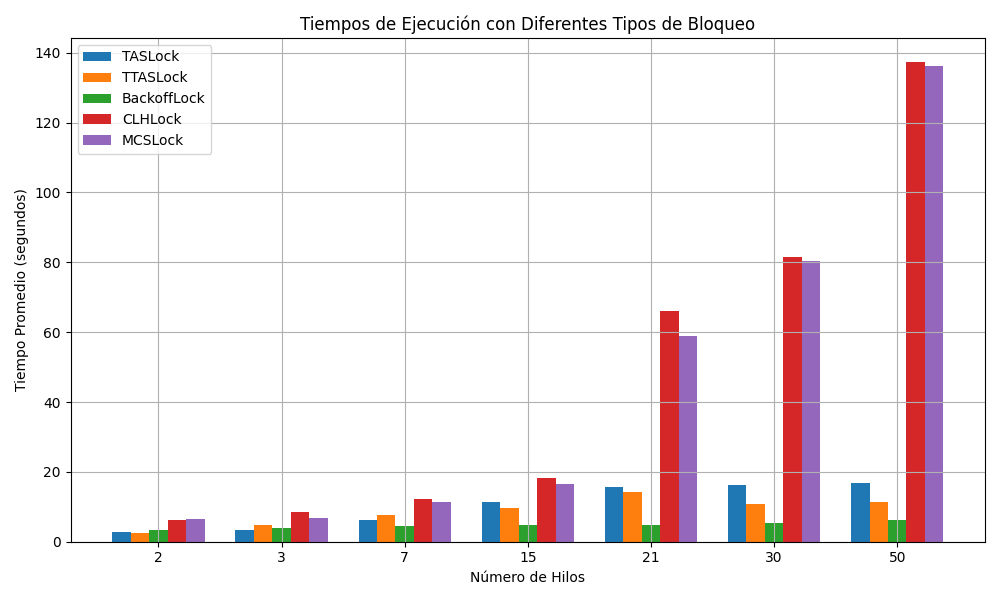
\includegraphics[width=1.0\linewidth]{Practica3/ImaP3/g1.png}
     \end{center}

\item Luz:

   \begin{center}
         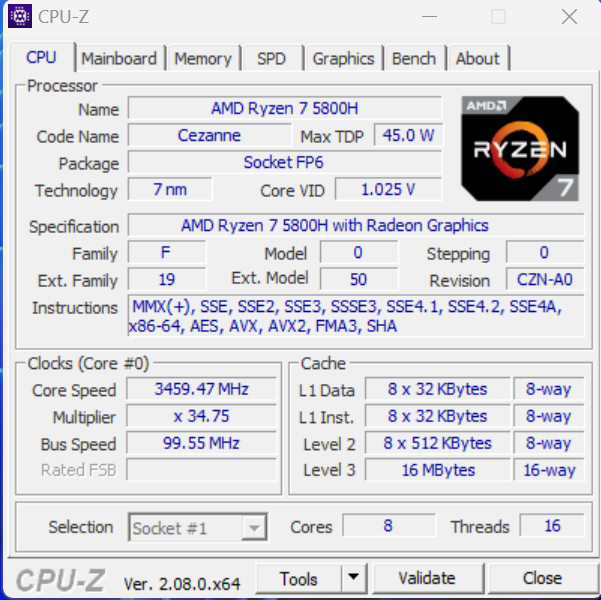
\includegraphics[width=0.6\linewidth]{Practica3/ImaP3/cpu.png}
     \end{center}
      \begin{center}
         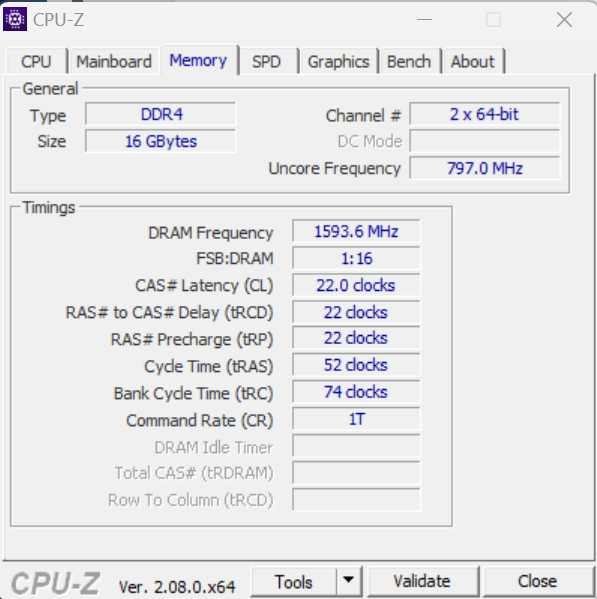
\includegraphics[width=0.6\linewidth]{Practica3/ImaP3/memoria.png}
     \end{center}
 \begin{center}
         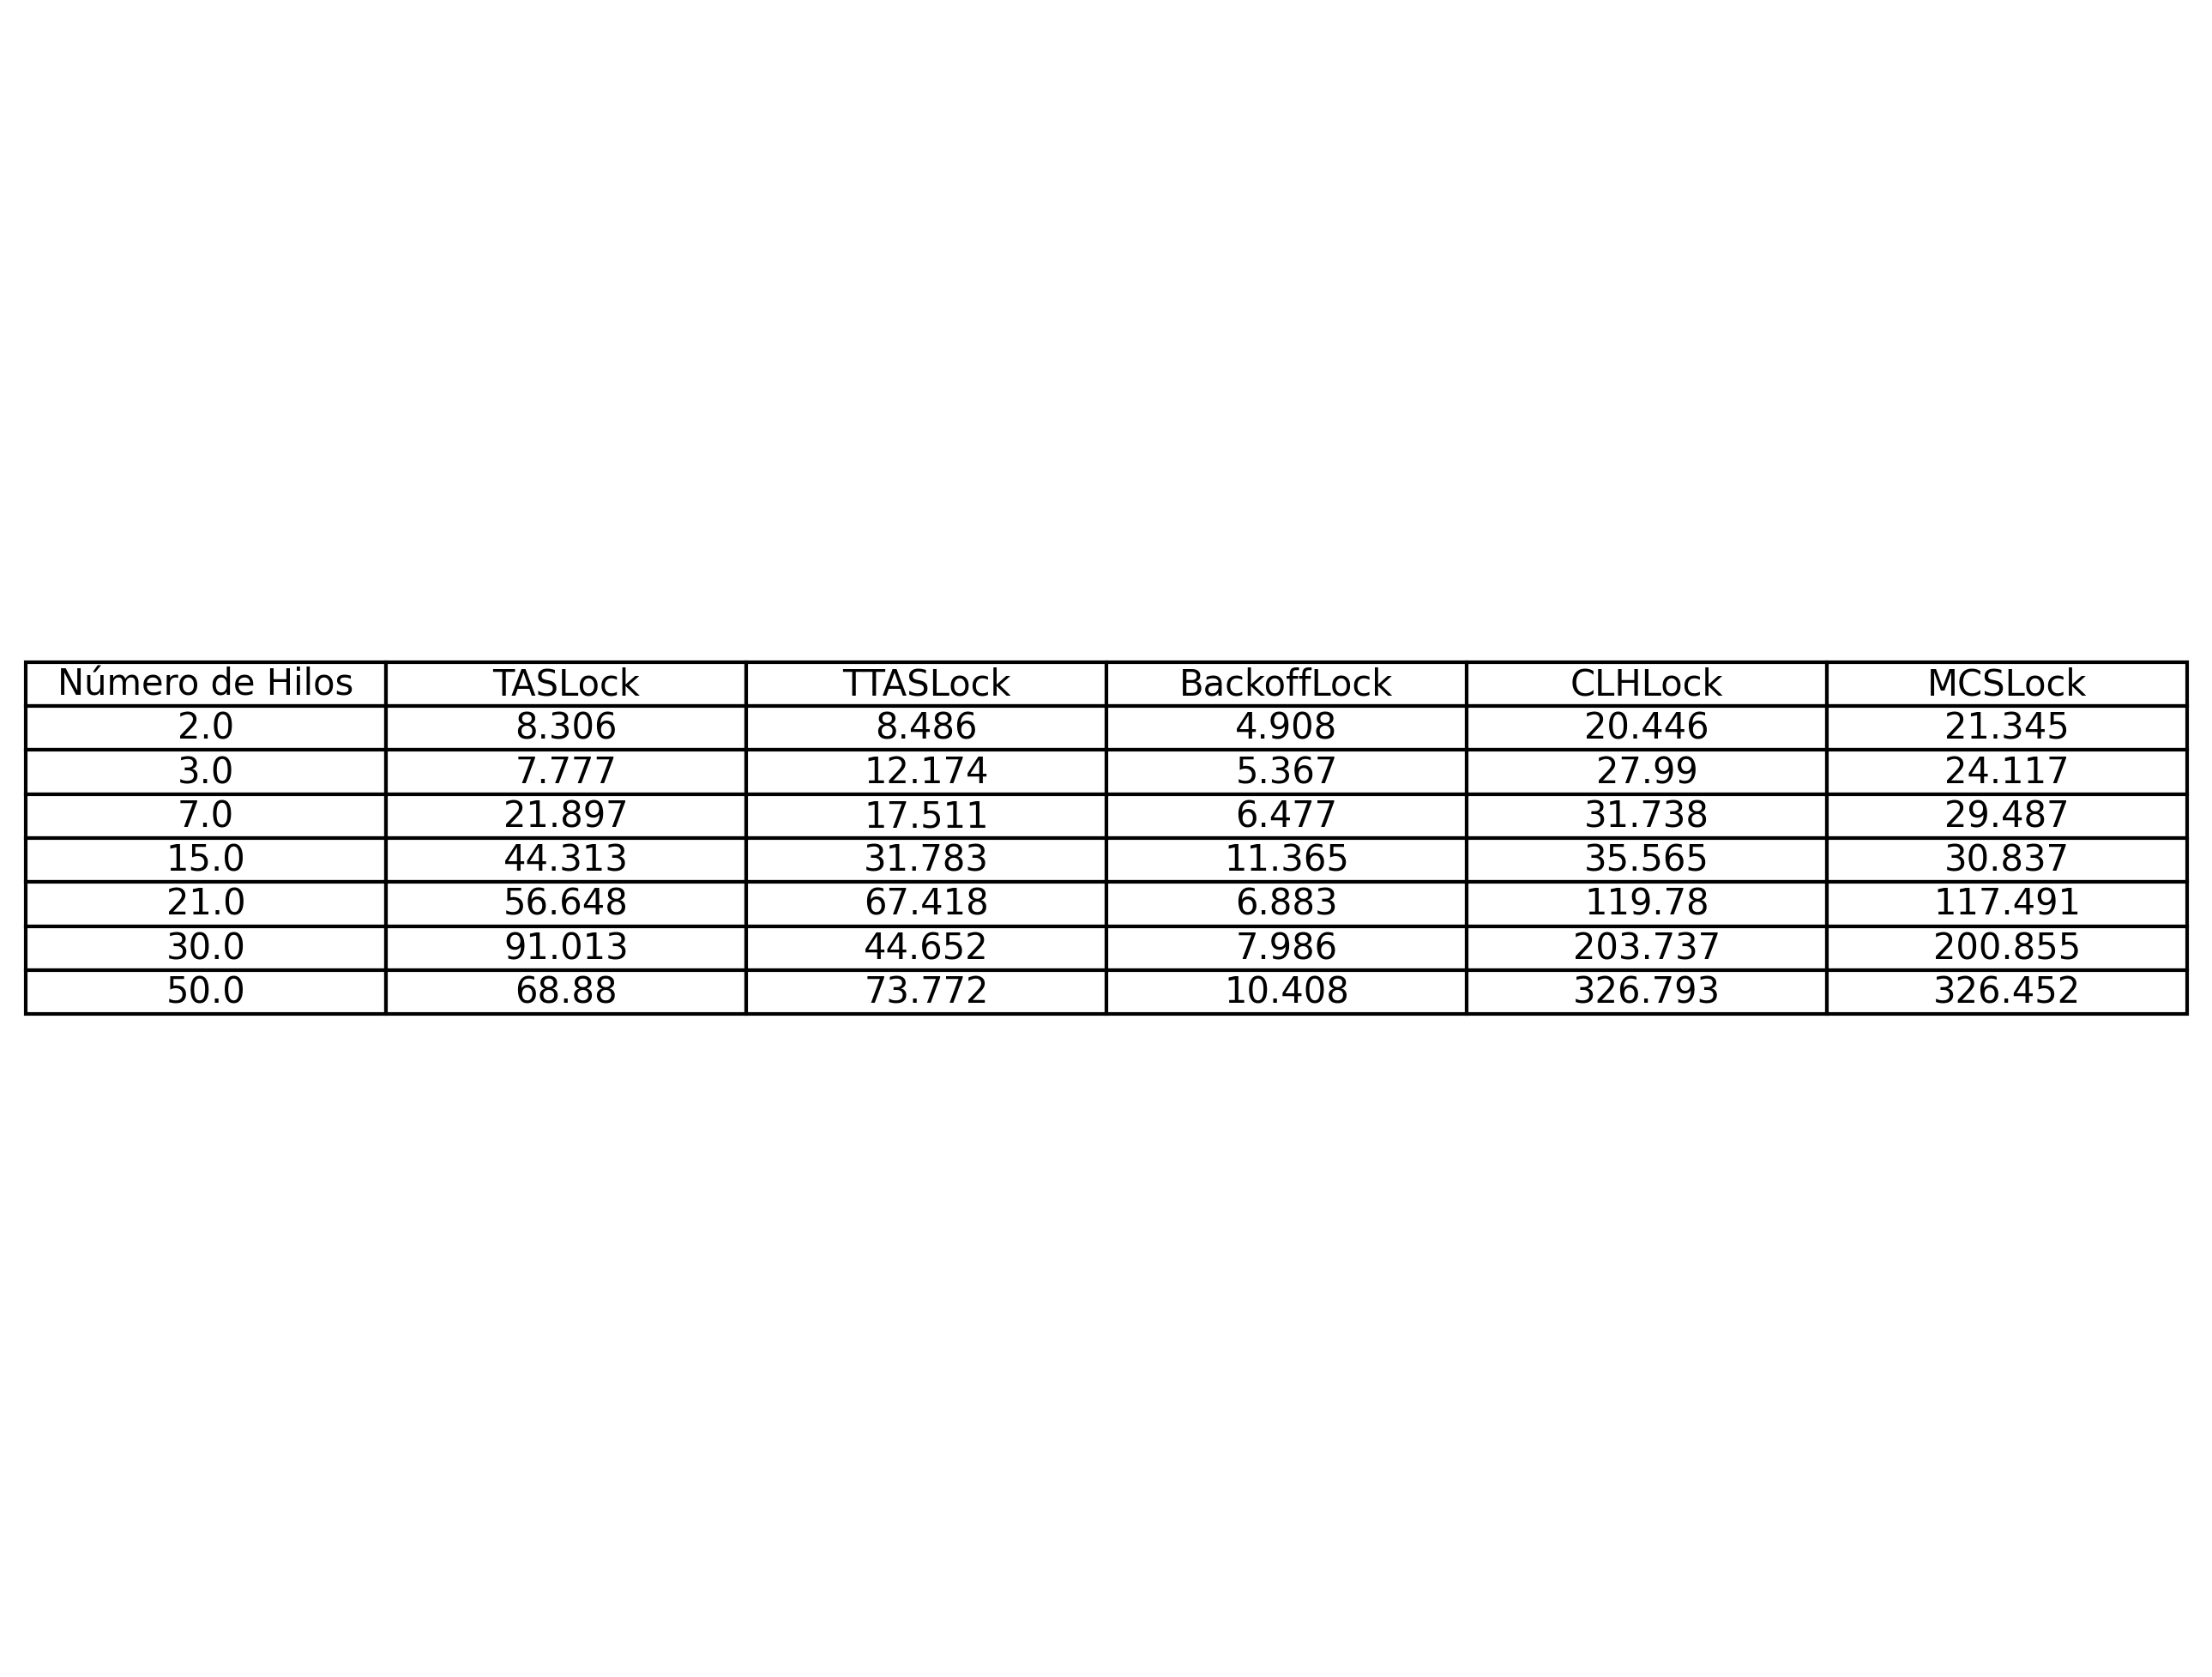
\includegraphics[width=1.0\linewidth]{Practica3/ImaP3/t2.png}
     \end{center}
     \begin{center}
         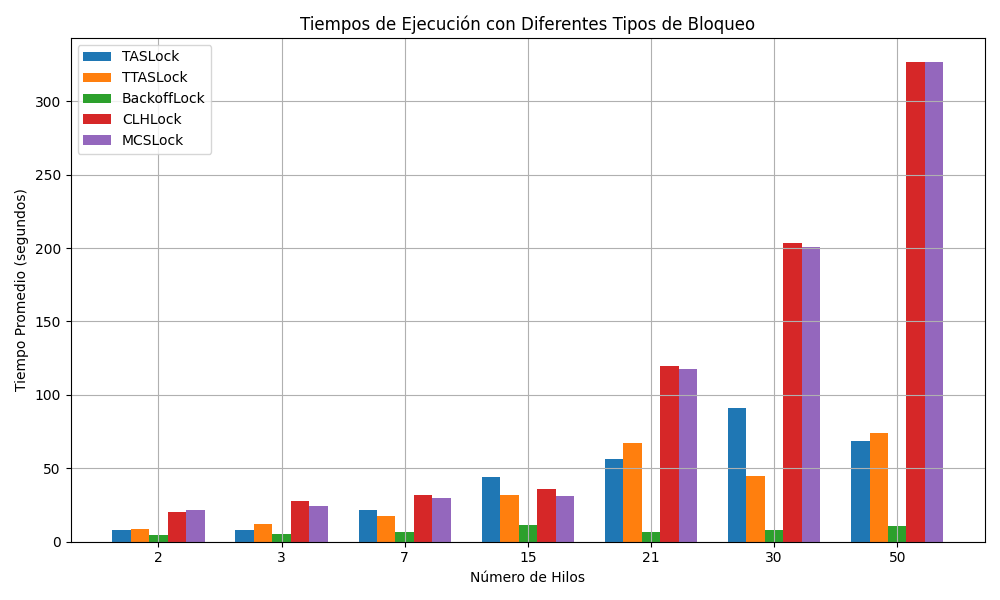
\includegraphics[width=1.0\linewidth]{Practica3/ImaP3/g2.png}
     \end{center}
\item Fernando:
\begin{center}
    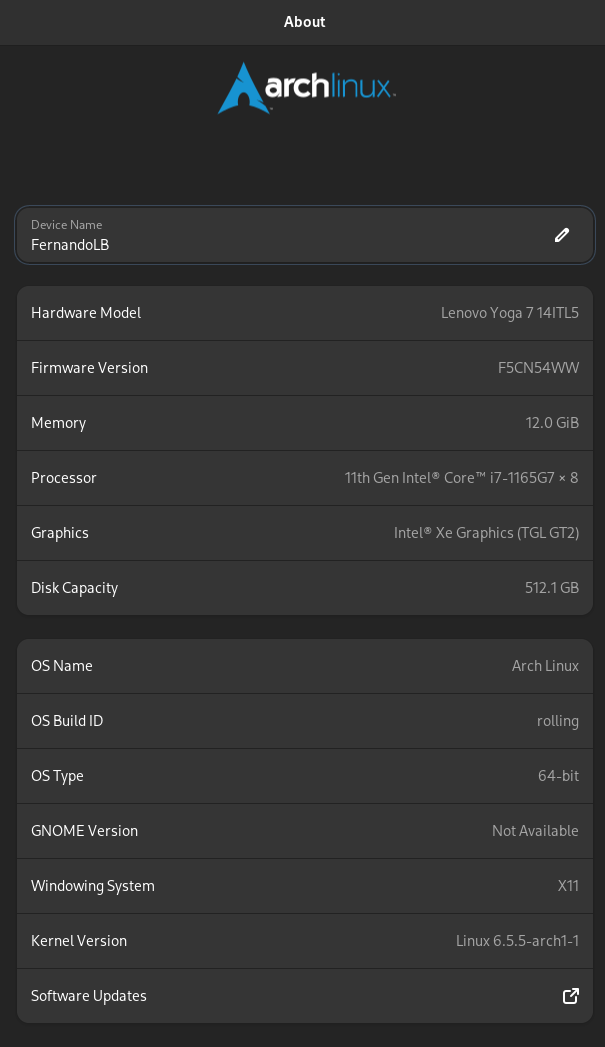
\includegraphics[width = 8cm]{Practica3/ImaP3/EspecificacionesFernando.png}
\end{center}
\begin{center}
         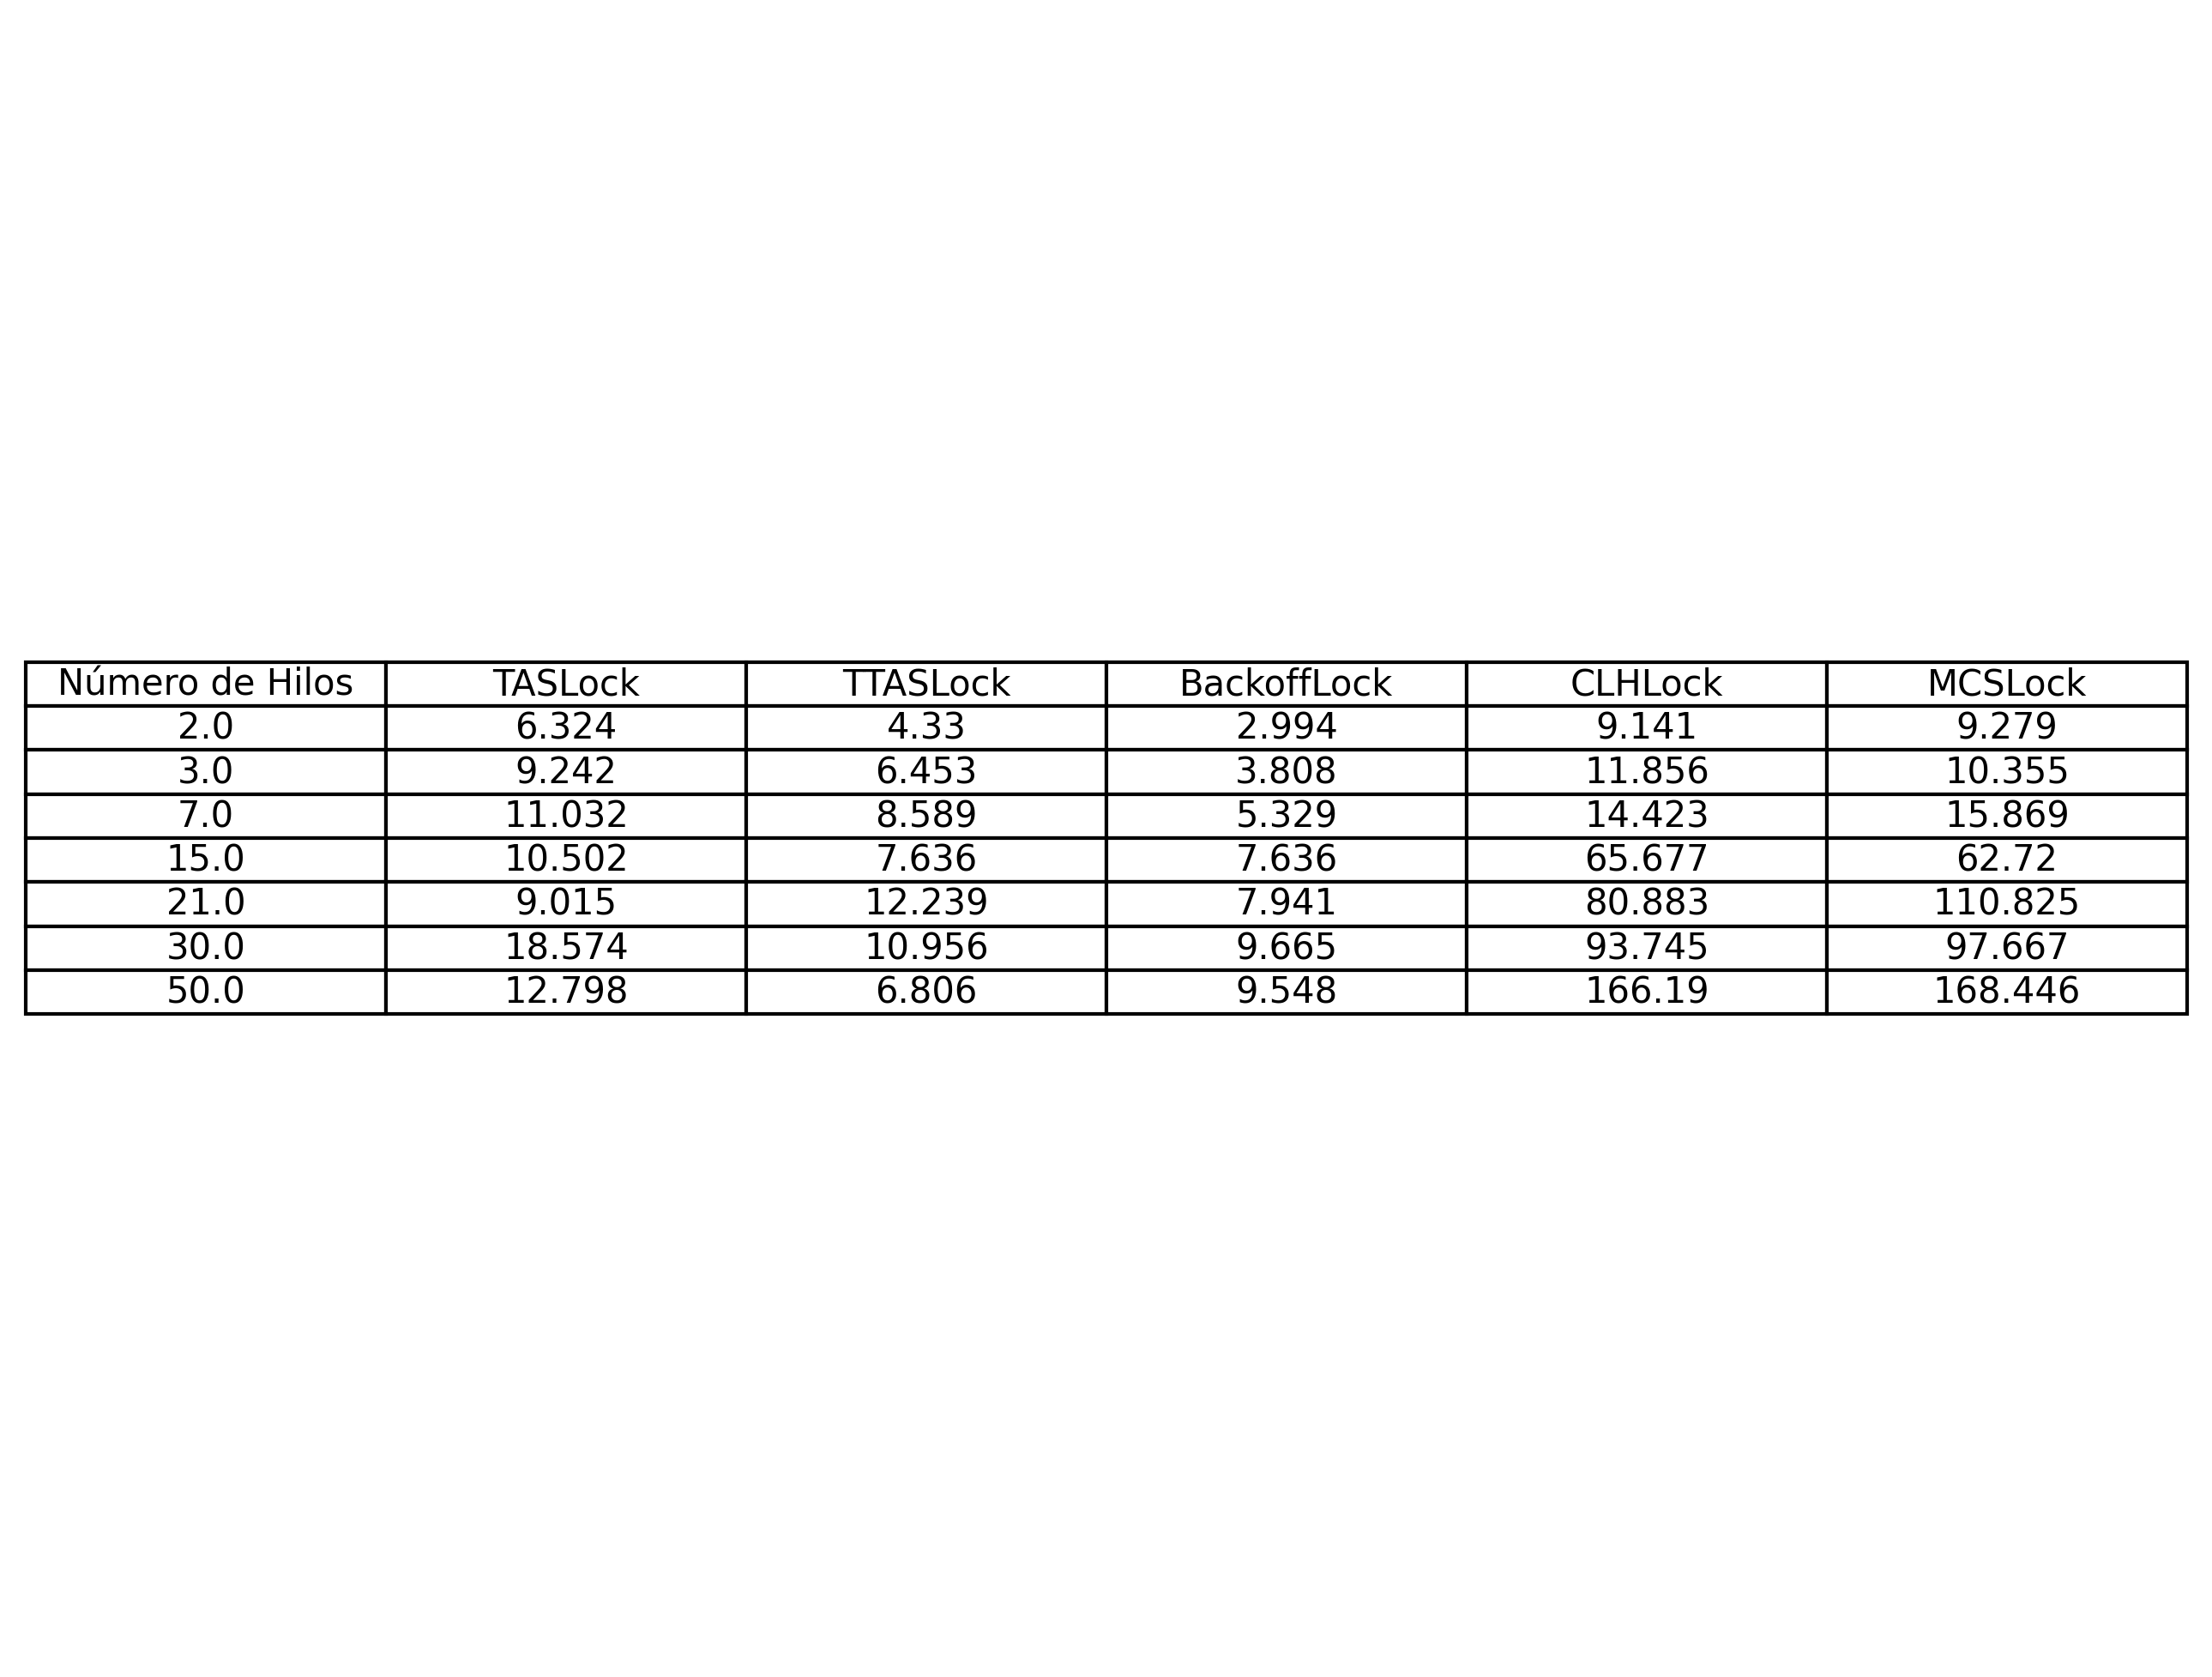
\includegraphics[width=1.0\linewidth]{Practica3/ImaP3/t3.png}
     \end{center}
        \begin{center}
         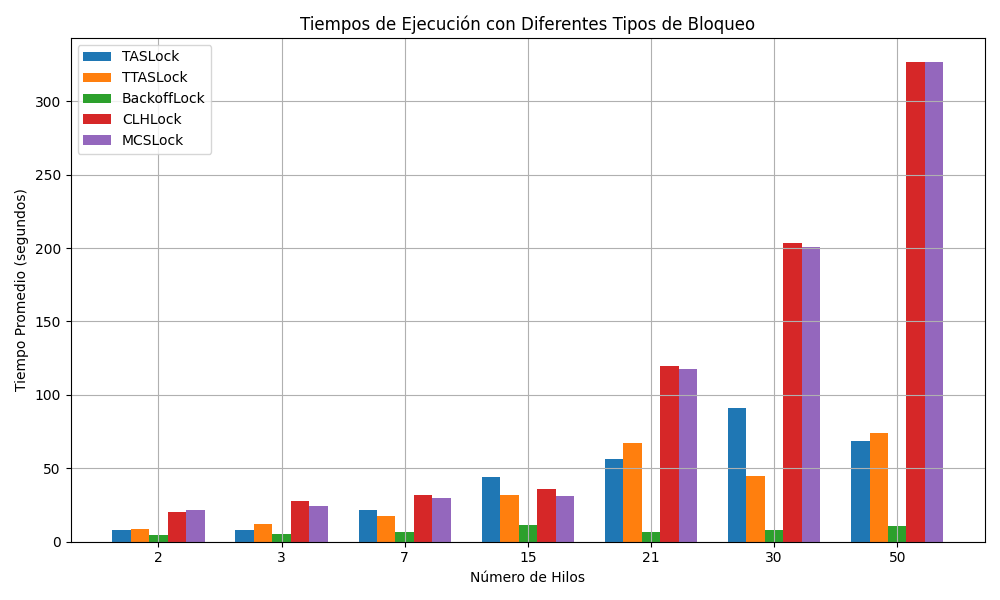
\includegraphics[width=1.0\linewidth]{Practica3/ImaP3/g2.png}
     \end{center}
 \end{itemize}

 \textbf{Porque se obtienen esos tiempos:}\\

 
Como podemos ver en las gráficas los que mas tarda son CLH y TLC se obtienen debido a la eficiencia de la gestión de bloqueos y la competencia por el recurso compartido además de que es muy importante el di positivo que estemos usando ya que algunos dispositivos pueden ejecutar con mayor potencia logrando menos tiempo en el caso de CLH s tardado debido a que usa una cola de nodos en la que los hilos se enfilan para adquirir el bloqueo en cambio los mas rapidos como TAS y TTAS no hace esto.

  \textbf{Compara el resultado:}\\

  
Comparando los resultados podemos notar que son muy similares pero los resultados obtenido por Gustavo son mas cortos en la mayoría de los casos esto se debe a que puso su computadora en la opción Perfonmance tuning que es una opción en los dispositivos Huawei , esta opción lo que hace es acelerar el procesador para que de su máximo rendimiento.


En el caso de luz podemos notar que tuvo tiempos mas tardados incluso con un procesador mas actual que el de Gustavo , sus resultados se deben a que tenia su dispositivo en ahorro de batería lo que limita a su procesador.

Otro factor que puede afectar los tiempos de ejecución puede ser el sistema operativo , como podemos notar Fernando usa Kali Linux y tiene en ocasiones mejores tiempos .


\textbf{Lo aprendido durante la practica y las impresiones recibidas al realizarla:}\\


Con esta practica hemos aprendido mucho sobre los mecanismos de bloqueo que se ocupan en la computación concurrente además de como usar diferentes estrategias de bloqueo , igual como los tiempos de ejecución pueden variara demasiado dependiendo la implementación realizada y el equipo que estemos usando  y como algunos mecanismos son más adecuados para escenarios con alta competencia por recursos, mientras que otros son más eficientes en situaciones con menos competencia y asi la elección del mecanismo de bloqueo correcto depende de la aplicación y sus requisitos de concurrencia. 

Nos impresiono como la elección del mecanismo de bloqueo correcto puede tener una gran diferencia en el rendimiento y la eficiencia de una aplicación.


\newpage

\section*{Referencias}
\begin{itemize}
    \item GeeksforGeeks. (2022). Java concurrency yield sleep and join methods. GeeksforGeeks. Recuperado de: \url{https://www.google.com/amp/s/www.geeksforgeeks.org/java-concurrency-yield-sleep-and-join-methods/amp/}

     \item  AtomicInteger (Java Platform SE 8 ). (2023, 14 junio).  Recuperado de: \url{https://docs.oracle.com/javase/8/docs/api/java/util/concurrent/atomic/AtomicInteger.html}
    

      \item  Jain, D., \& Jain, D. (2023). An introduction to atomic variables in Java | Baeldung. Baeldung.  Recuperado de: \url{https://www.baeldung.com/java-atomic-variables}


     
\end{itemize}

\end{document}